%\documentclass[10pt,conference]{IEEEtran}
%\documentclass[9pt,conference]{sig-alternate}
%\documentclass[9pt,conference]{sig-alternate}
%\documentclass[10pt,print,letterpaper,nocopyrightspace]{sigplan-proc-varsize}
\documentclass[10pt,print,letterpaper]{sigplan-proc-varsize}

\usepackage{amsmath,epsfig}
\usepackage{url}
\usepackage{xspace}
\usepackage{colortbl}
\usepackage{subfigure}
\usepackage{dsfont}
\usepackage{boxedminipage}
\ifx\pdfoutput\undefined
\usepackage[hypertex]{hyperref}
\else
\usepackage[pdftex,hypertexnames=false]{hyperref}
\fi

\usepackage{amssymb}
\usepackage{wasysym}
\usepackage[left=2.54cm,top=2.54cm,right=2.54cm,bottom=2.54cm,nohead,nofoot]{geometry}



\DeclareMathOperator*{\argmax}{argmax}
%\usepackage{times}

\def\ucb{$^{\dagger}$}
\def\stanford{$^{\ddagger}$}
\def\arch{$^{\star}$}

\newcommand{\kb}{kB}
\newcommand{\rene}{Ren{\'e}\xspace}
\newcommand{\reneii}{Ren{\'e}2\xspace}
\newcommand{\wec}{WeC\xspace}
\newcommand{\mica}{Mica\xspace}
\newcommand{\micaii}{Mica2\xspace}
\newcommand{\micaz}{MicaZ\xspace}
\newcommand{\micadot}{Mica2Dot\xspace}
\newcommand{\iic}{I$^2$C\xspace}
\newcommand{\uA}{$\mu$A\xspace}
\newcommand{\dotmote}{Dot\xspace}
\newcommand{\mhz}{MHz\xspace}
\newcommand{\ghz}{GHz\xspace}
\newcommand{\kbps}{kbps\xspace}
\newcommand{\dsn}{DSN\xspace}
\newcommand{\io}{I/O\xspace}
\newcommand{\telos}{Telos\xspace}

\newcommand{\T}{\mathds{T}}
\newcommand{\XXXnote}[1]{{\bf\color{red} XXX: #1}}


\begin{document}

%\conferenceinfo{Sensys'08,} {November 5--7, 2008, Raleigh, NC, USA.}  
%\CopyrightYear{2008} 
%\crdata{978-1-60558-096-8/08/09} 

\title{Towards Empirically-Driven Verification in Buildings}
%\numberofauthors{1} 
%\author{\alignauthor Stephen Dawson-Haggerty, Jorge Ortiz, Xiaofan Jiang and David Culler\\
%\affaddr{Computer Science Division}\\
%\affaddr{University of California, Berkeley} \\ 
%\affaddr{Berkeley, California 94720} \\
%\email{\{stevedh,jortiz,xjiang,culler\}@cs.berkeley.edu}
%} 


%\subtitle{Paper \# Insert Reg Number Here}

%\title{Alternate {\ttlit ACM} SIG Proceedings Paper in LaTeX
%Format\titlenote{(Produces the permission block, and
%copyright information). For use with
%SIG-ALTERNATE.CLS. Supported by ACM.}}
%\subtitle{[Extended Abstract]
%\titlenote{A full version of this paper is available as
%\textit{Author's Guide to Preparing ACM SIG Proceedings Using
%\LaTeX$2_\epsilon$\ and BibTeX} at
%\texttt{www.acm.org/eaddress.htm}}}
%
% You need the command \numberofauthors to handle the 'placement
% and alignment' of the authors beneath the title.
%
% For aesthetic reasons, we recommend 'three authors at a time'
% i.e. three 'name/affiliation blocks' be placed beneath the title.
%
% NOTE: You are NOT restricted in how many 'rows' of
% "name/affiliations" may appear. We just ask that you restrict
% the number of 'columns' to three.
%
% Because of the available 'opening page real-estate'
% we ask you to refrain from putting more than six authors
% (two rows with three columns) beneath the article title.
% More than six makes the first-page appear very cluttered indeed.
%
% Use the \alignauthor commands to handle the names
% and affiliations for an 'aesthetic maximum' of six authors.
% Add names, affiliations, addresses for
% the seventh etc. author(s) as the argument for the
% \additionalauthors command.
% These 'additional authors' will be output/set for you
% without further effort on your part as the last section in
% the body of your article BEFORE References or any Appendices.

\numberofauthors{2} %  in this sample file, there are a *total*
% of EIGHT authors. SIX appear on the 'first-page' (for formatting
% reasons) and the remaining two appear in the \additionalauthors section.
%
\author{
% You can go ahead and credit any number of authors here,
% e.g. one 'row of three' or two rows (consisting of one row of three
% and a second row of one, two or three).
%
% The command \alignauthor (no curly braces needed) should
% precede each author name, affiliation/snail-mail address and
% e-mail address. Additionally, tag each line of
% affiliation/address with \affaddr, and tag the
% e-mail address with \email.
%
% 1st. author
\alignauthor
%Prabal Dutta\\
%       \affaddr{Computer Science Division}\\
%       \affaddr{Univ. of California, Berkeley}\\
%       \affaddr{Berkeley, CA 94720}\\
%       \email{prabal@cs.berkeley.edu}
% 2nd. author
%\alignauthor
%David Culler\\
%       \affaddr{Computer Science Division}\\
%       \affaddr{Univ. of California, Berkeley}\\
%       \affaddr{Berkeley, CA 94720}\\
%       \email{culler@cs.berkeley.edu}
% 3rd. author
%\alignauthor
%Scott Shenker\\
%       \affaddr{Computer Science Division}\\
%       \affaddr{Univ. of California, Berkeley}\\
%       \affaddr{Berkeley, CA 94720}\\
%       \email{shenker@cs.berkeley.edu}
%}
me and me\\
       %\affaddr{Department}\\
	\affaddr{University of California, Berkeley}\\
       %\affaddr{Institution}\\
       %\affaddr{City, State Zip}\\
       \email{\{me,you\}@eecs.berkeley.edu}
}


\maketitle

%\date{14 April 2007}
%\maketitle

\begin{abstract}
% Buildings represents one of the richest sensor-enriched environments in the world and
% have become a prime target for energy efficiency.  Work in this area is moving much of
% the monitoring and control tasks to software, to make use of the sensor data.  However,
% the metadata -- used to determine the context of stream -- is manually specified and often
% changes as the building itself evolves.  This distributed information gathering and update
% process is manual and error-prone.  As such, it has become necessary to verify the metadata
% is an automatic fashion.  This paper examines several empirical techniques for verifying various
% kinds of contextual relationships, namely spatial and categorical.  We show how mode decompisition
% can be used to find spatial relationships among sensor streams under certain conditions; doing a
% significantly better job that working with the raw data feeds.  In addition, we show how categorical
% separation can be achieved through supervised learning and offer techniques for dealing with 
% large fractions of missing data -- a fundamental issue sensor-data analysis.


Large buildings contain a rich sensing fabric used for monitoring and control.
With the increased interest in energy efficiency, buildings are becoming more reliant on software processes
to automate control and analytics of the associated sensor data.  These processes rely on the sensor data's
metadata in order obtain the necessary feeds for analysis.  However, the metadata is manually entered and 
does not change with the evolution of the building.  Furthermore, manual maintenance does not scale as the number
of sensors increase with the size of the building.  %An automated verification process is needed.
This paper examines several empirical techniques for verifying various
kinds of contextual relationships, namely spatial and categorical.  We examine three building traces which contain
more than a year of data, over 1500 streams, and 63 type-labels.
We show how mode decomposition
can be used to uncover spatial relationships among sensor streams, where the raw data give no information.
In addition, we show how categorical and placement  
separation can be achieved through supervised learning and offer techniques for dealing with 
large fractions of missing data -- a fundamental issue in sensor-data analysis.


\end{abstract}

% A category with the (minimum) three required fields
%\category{B.0}{Hardware}{General}
%\category{B.4}{Hardware}{Input/Output \& Data Communication}

%\terms{Design, Implementation, Performance, Experimentation}

%\keywords{Churn, Link, Routing, Wireless, Sensor Network, Mote}

%\newpage

\section{Introduction}
\label{sec:intro}


% \begin{itemize}
% \item Buildings are relying more and more on software 
% \item Software relies on sensors; uses metadata to contextualize the data
% \item Metadata is inputted by human, error-prone; changes over time, becomes stale.
% \item This is perhaps not very common in a single building, but huge problem at scale.
% \item automatic verification is necessary
% \item three types: categorical, spatial, functional
% \item we show how much of each we can get emprirically on the first two; prior work handles functional.
% \end{itemize}

% Buildings represent some of the largest deployments of sensors on physical infrastructure.  Traditionally used
% for historical analysis and supervisory control, these sensors are being used more and more for software-based, model-driven
% control and sophisticated real-time analytics.  The notion of smart buildings consists of a dense deployment of
% sensors in systems and spaces of the building combined with sophisticated software that uses the data collected
% from the deployment to intelligently control and aggregate the information to provide greater insight into the 
% dynamics and pathologies of buildings.  Since buildings consume a large fraction of the energy produced
% in many countries around the world~\cite{}, the move towards smart buildings is accelarating~\cite{}.

% There has been lots of recent work in this area~\cite{BOSS, FIAP, smap, ucsd, bacnetip}

Buildings have become a prime target for cyber-physical systems research, as they consume 40\% of
the energy in the U.S.~\cite{EIA}, are poorly understood,
and offer a rich sensing infrastructure.  Thousands of sensors are embedded throughout 
the building and produce periodic physical measurements. In order to interpret the information, metadata describing 
the placement of sensors is recorded.
However, deployments and their metadata are configured manually.  As such, they are prone to human error.
Moreover, over time sensors are replaced and the physical configuration of the building changes -- walls removed,
new offices set up -- but the metadata describing the new locations are not.  This leads to analytical errors in processes 
that rely on the metadata when interpretting sensor feeds.  For example, model-predictive control processes rely
on the sensors in a specific room or floor~\cite{MPC}.  Because of the size and distributed nature of the deployment, 
it is cumbersome, error-prone, and impractical to maintain accurate metadata about sensor placement over time.  An
automatic processes is needed.

Sensor metadata contains information about the sensor and its context.  It usually units of measure, 
the room it is in, and the system it helps feed.  For example, consider the point name `SODA1R465B_ART'.
\emphSODA1 refers to air-handling unit 1 on soda hall, \emph{R465B} says the sensor is in room 465B, and \emph{ART}
denotes arear-room temperature.  Although not explicitly a unit of measure, the associated data is recorded in degrees
fahrenheit.

Sensor placement information is typically embedded in the name or associated metadata for each sensor in the building.
These are used to group sensors by location.  For example, in our building data, all sensors that contain the string
 `410' in their name are in room 410.  Processes typically group streams in this fashion: using regular-expression matching 
or field-matching queries on the characters in the sensor name or metadata.  If these are not updated to reflect changes
then such group-by query results will not accurately represent true spatial relationships.  
Fontugne et al.~\cite{IOT} observe that spatial associations can be derived empirically.  We start with this approach in our 
work and explore, more deeply, the extent to which it can be used 
as a verification tool for corroborating the groups constructed from character-matching queries.  We refer
to this process as \emph{spatial verification}.

Prior work~\cite{IOT} makes use of a technique called Empirical Mode Decomposition (EMD)~\cite{EMD} to statistically cluster correlated
usage patterns.  Sensors close to each other show strong statistical correlations while sensors further apart show weaker correlations.  
The main parameter in their approach, the correlation threshold, is explored to demonstrate how it relates to characteristic spatial patterns
 in the sensor feeds.  However, they do not characterize the threshold as it relates to physical configuration.
Fontugne et al.~\cite{SBS} expand the work by applying EMD to uncover functional device patterns.  They develop
an unsupervised learning method to model normal usage patterns and apply an anomaly detection algorithm to alert when patterns
have deviated from the norm.  The methodology used in their work divides raw signals into four separate frequency bands
and shows the medium band to carry the most spatial information.

In this paper, we explore the threshold parameter in~\cite{IOT} more deeply, in order to move towards automatic spatial clustering, 
to be used as a form of verification. We use EMD and the intrinsic mode function (IMF) re-aggregation methodology described in~\cite{SBS}, with some modifications, to statistically analyze the threshold parameter
and its relationship to spatial separation in a building.  We explore the hypothesis that \emph{a statistical boundary, analogous to a physical one,
exists and is empirically discoverable}.
We conduct an empirical analysis on the data collected from 15 sensors in 5 rooms over a one-month period.  Our study makes the following contributions:

\begin{itemize}
\item We corroborate the results in~\cite{IOT}, verifying the spatial correlation pattern in a very different building.
\item We characterize the correlation coefficient (corrcoeff) distribution of sensors in the same room and different rooms and validate our existence hypothesis for this preliminary sample.
\item We demonstrate that the statistical boundary between sensors in various rooms converges to a similar value and this value generalizes across rooms in this study.
\item We show the tradeoff between the true and false positive rate inherent to threshold selection. We also show that our method improves the classification accuracy from 80\% to 93.3\%.
\end{itemize}

Our results are promising yet preliminary.  We are able to find a statistical separation across a small number of rooms, quite well.
Our study, however, does not explore the extent to which the physical separation affects the results.  Certainly for rooms that
are far apart we observe a statistical distinction using our methodology.  However, we also find that in some cases, our approach
does not work as well.  We discuss the approach and results in the rest of the paper, followed by a short discussion and future work.




\begin{itemize}
\item Buildings are relying more and more on software 
\item Software relies on sensors; uses metadata to contextualize the data
\item Metadata is inputted by human, error-prone; changes over time, becomes stale.
\item This is perhaps not very common in a single building, but huge problem at scale.
\item automatic verification is necessary
\item three types: categorical, spatial, functional
\item we show how much of each we can get emprirically on the first two; prior work handles functional.
\end{itemize}

\newpage

\section{Related Work}
\label{sec:related}

There has been much research work on sensor stream clustering and trace analysis. Chen and Tu~\cite{DStream} investigate 
how to cluster data streams in real-time using a density-based approach with a two-tiered framework. The first tier captures 
the dynamics of a data stream with a density decaying technique and then maps it to a grid.  The second tier computes a grid 
density based on how it clusters the grid. Their approach differs from ours in that they focus on decreasing algorithm 
complexity for real-time sensor stream clustering.  We run our analysis on historical traces and use correlation analysis
in our clustering algorithm.

Kapitanova et al.~\cite{failure} describe a technique to monitor sensor operations in the home and identify sensor failures. 
The classifier is trained on historical sensor data to obtain the relationship between sensors, assuming the number and location of 
sensors is known.  When a failure or removal of a sensor occurs, the classifier's behavior deviates and the event is captured. Our method does not require any prior knowledge and instead tries to cluster feeds to discover their relative placement.

Lu and Whitehouse~\cite{blueprints} formulate a new algorithm, particularly leveraging the semantic constraints interpreted from sensor 
data to determine sensor locations. The algorithm identifies how many rooms are present using motion sensors and determines room position based on physical constraints. Finally, it maps each sensor into the associated room. Our efforts focus on using intrinsic patterns typically pre-existing in building system sensor feeds to uncover physical relationships.

Fontugne et al.~\cite{IOT} propose a new method to decompose sensor signals with EMD.
They extract the intrinsic usage pattern from the raw traces and show that sensors close to each other have higher intrinsic correlation. However, they do not explore the observation more deeply by answering whether there is a statistically discoverable boundary between sensor clusters in different rooms, or if there is a uniform threshold in the correlation coefficients able to be generalized to different rooms.

Fontugne et al.~\cite{SBS} carry on the work and propose an unsupervised method to monitor sensor behavior in buildings. They constructed 
a reference model out of the underlying pattens, obtained with EMD,  and use it to compare future activity against it.  They report an anomaly whenever a device deviates from the reference. This work exploits EMD as a method to detrend the signals and capture the inter-device relationships.

Much work utilizes EMD on medical data~\cite{ecg}, speech analysis~\cite{speech}, image processing~\cite{ip} 
and climate analysis~\cite{climate}. Our method adopts EMD to determine whether a discoverable statistical boundary exists in sensors traces
from sensors in different rooms and whether such a boundary
 can be generalized across rooms with various kinds of sensors.


\newpage

\section{Sensor Data In Buildings}
\subsection{Software-based Analysis and Control}
\subsection{Model-Predictive Control}
\subsection{Contextualizing Sensor Data}
\subsection{Labeling Errors And Building Evolution}

\newpage

\section{Empirical Verification}
\subsection{Spatial, Categorical, and Functional}
\subsection{Challenges}

\newpage

% \section{Contention Experiment}

%\begin{figure*}[t]
%\begin{center}
%\includegraphics[width=\columnwidth]{../figs/tdma_throughput}
%\caption{Measured throughput for TDMA protocol. We expected the throughput to be low for lower probabilities of collision because of the smaller possibility of successful packet reception. However, we did not expect TDMA to have a peak at a collision probability of 0.25}
%\label{tdma_through}
%\end{center}
%\end{figure*}


%\subsection{Experimental Set-up}

%\begin{equation}
%\label{col-eqn}
%P_{col} = P_{s1}*P_{s2}
%\end{equation}


\section{Results}

% \subsection{Spatial Properties}

% \begin{enumerate}
% \item Window/less
% \item Orientation (North/South facing)
% \item Separation of characteristically different rooms.
% \end{enumerate}

% \subsubsection{Methdology}

% \subsubsection{Results}
% \begin{figure*}[ht!]
% \centering
% 	\begin{subfigure}{0.48\textwidth}
%                 \centering
% 		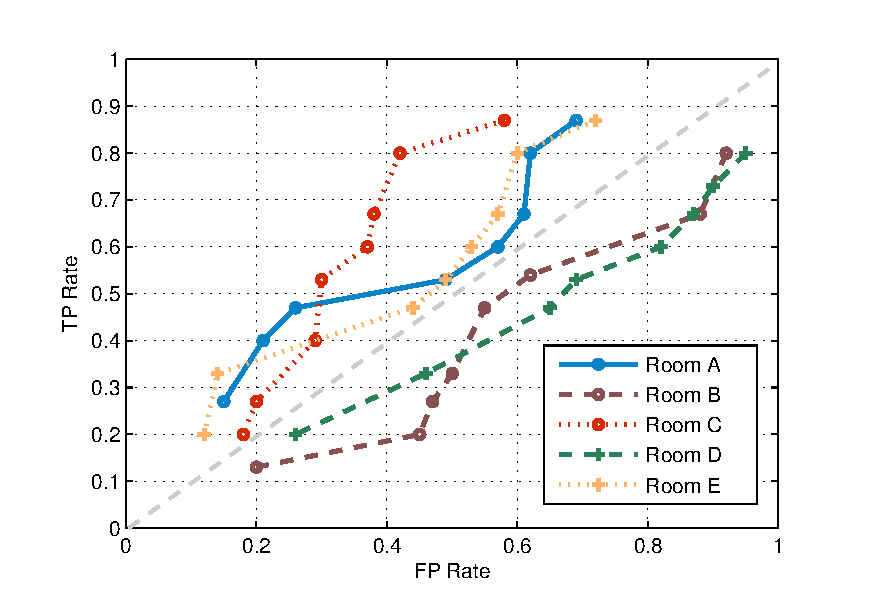
\includegraphics[width=\textwidth]{./fig/ROC_bsln.eps}
%                 \caption{Correlating the raw signals.}
% 	\end{subfigure}
% 	\begin{subfigure}{0.48\textwidth}
%                 \centering
% 		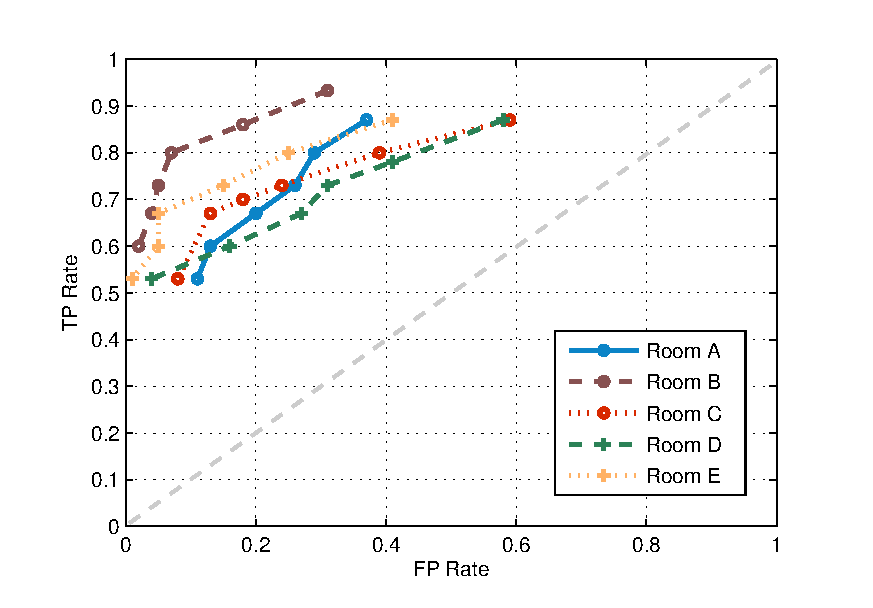
\includegraphics[width=\textwidth]{./fig/ROC_new.eps}
%                 \caption{Correlating the re-aggregated IMFs in the ``medium'' frequency band.}
%                 \label{fig:rocA}
% 	\end{subfigure}
% \caption{The ROC curves depict the sensitivity of the raw signal and mid-frequency IMFs to the threshold value. We choose the 0.2 FPR point as the boundary threshold for each room. }
% \label{fig:roc}
% \end{figure*}

% \section{Experimental Results}
% We conduct two sets of experiments. First, we quantify the sensitivity of our method for different threshold values 
% and examine the effect of different time spans on the threshold. We then cluster the traces based on our threshold analysis 
% and compare it with a baseline approach using multidimensional scaling and k-means.
% % as well as with an approach combining multidimensional scaling and k-meas. 
% % Last, we validate the usefulness of the proposed method in a case study.

% \subsection{Experimental Setup}
% \begin{figure}[h!]
% \centering
%   \includegraphics[width=0.45\textwidth]{./figs/SDH3_crop}
% \caption{We collect data from 15 sensors in 5 rooms sitting on 4 different floors. This is a map of a section of the 3rd floor
% in Sutardja Dai Hall.}
% \label{fig:sdh}
% \end{figure}

% We perform an empirical study on sensor data collected from 15 sensors across 5 rooms on 4 different floors of a large building, as detailed in Table~\ref{table:roomspec}. 
% Each room has three sensors: a temperature sensor, a $CO_{2}$ sensor,  and a humidity sensor. 
% The data from these is reported to an sMAP~\cite{smap} archiver. The data set used comes from a deployment~\cite{Jay} lasting 
% over 6 months on several floors in Sutardja Dai Hall (SDH) at UC Berkeley, where one sensor box -- which contains a thermometer, a humidity sensor and a $CO_{2}$ sensor -- is placed in each room. The box reports data over 6LowPAN~\cite{6lowpan} to a sMAP archiver every 15 seconds. 
%  % The other is a long-term deployment comprised of thousands of sensors that are part of the Building Management System (BMS).
%  % We choose the portion of the SDH data set where the sensor devices, accessible via BACnet~\cite{BACnet}, report data to the archiver every 
%  %few minutes. 
%  Due to intermittent data loss, we pick a time span without interruption, starting in January until mid-Feburary, 2013, for evaluation.

% \begin{table}[ht!]
% \caption{Room Specs}
% \centering % used for centering table
% \begin{tabular}{c c c c}% centered columns (4 columns)
% \hline %inserts single horizontal lines
% Room\# & Orientation & Floor & Type \\ % inserts table 
% %heading
% \hline\hline % inserts double horizontal line
% A & West & 2 & Computer Lab \\ % inserting body of the table
% B & South & 4 & Conference Room \\
% C & No Window & 2 & Classroom \\
% D & North & 7 & Conference Room \\
% E & South & 5 & Conference Room \\ % [1ex] adds vertical space
% \hline %inserts single line
% \end{tabular}
% \label{table:roomspec} % is used to refer this table in the text
% \end{table}

% \subsection{Baseline and Metrics}
% % We exploit a simple approach as baseline to compare with our proposed approach: instead of computing the correlation coefficients between re-aggregated IMFs of sensor feeds, we directly use the raw sensor data to do the correlation analysis and generate the two distributions for thresholding approach evaluation similarly to what described previously.

% % As a baseline, we perform correlation analysis on the raw data. We generate two distributions, as previously described, and observe the effects of the choice of threshold on the true/false positive rate.
% As a baseline, after we generate the two distributions described previously, we apply multidimensional scaling (MDS) to the corrcoeff matrix, in order to transform the original high-dimensional relative space to a 3-D space with an absolute origin, and run the k-means clustering algorithm.
% We choose the true-positive rate (TPR, also known as recall rate) and false-positive rate (FPR) as metrics to evaluate the performance of our method versus the naive approach, which correlates the raw traces. A true-positive (TP) is when a sensor pair in a room is classified as being co-located 
% while a false-positive (FP) is when a sensor that is not in room is classified as being so.
% %is that a sensor not in room A is clustered as in room A.

% \begin{figure}[h!]
% \centering
% 	\includegraphics[width=0.45\textwidth]{./figs/Inter_intra_relationships}
% \caption{Two populations are examined for our threshold analysis.  A solid line connects sensors in the same room while a dotted line connects
%  to a pairs in different rooms.}
% \label{fig:group}
% \end{figure}

% \begin{figure}[h!]
% \centering
% 	% \begin{subfigure}{0.22\textwidth}
%  %                \centering
% 	% 	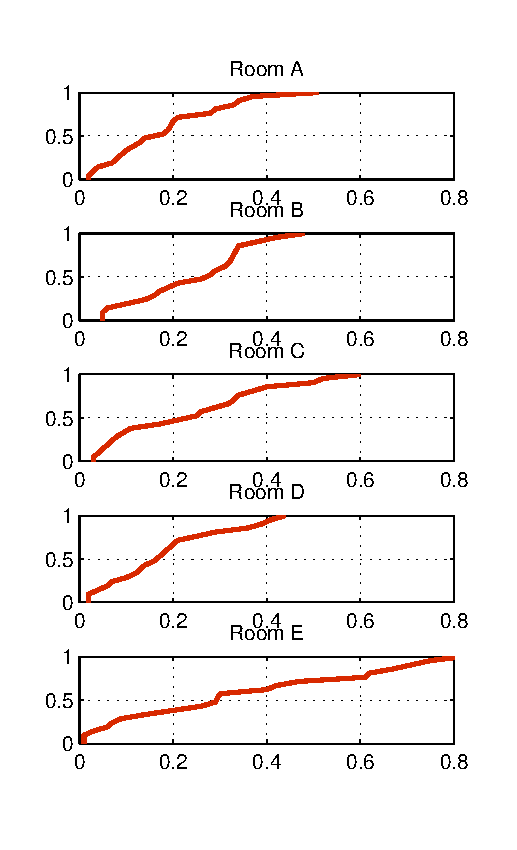
\includegraphics[width=\textwidth]{./fig/cdf_intra.eps}
%  %                \caption{Pairs in the same room}
%  %                \label{fig:cdf_intra}
% 	% \end{subfigure}
% 	% \begin{subfigure}{0.22\textwidth}
%  %                \centering
% 	% 	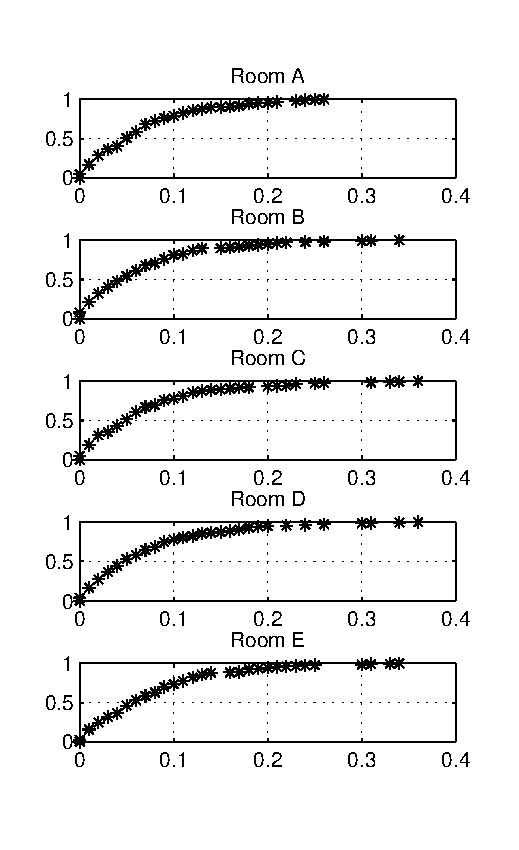
\includegraphics[width=\textwidth]{./fig/cdf_inter.eps}
%  %                \caption{Pairs in different rooms}
%  %                \label{fig:cdf_inter}
% 	% \end{subfigure}
% 	\includegraphics[width=0.45\textwidth]{./figs/corrcoeff_cdf_in_out}
% \caption{CDF of correlation coefficients between IMFs of sensor feeds: the dotted lines point to some threshold which divides
%  the distribution and produces a TPR and FPR.
% % (a) On average, the recall rate of clustering sensors inside one room is (0.62, 0.86). (b) The 80\% corrcoeffs between sensor feeds in rooms falls into (0.1, 0.12).
% }
% \label{fig:cdf}
% \end{figure}

% \subsection{Characterizing the Boundary}
% To corroborate our boundary-existence hypothesis, we first need to characterize the boundary between sensors in different rooms. 
% We compute the pairwise correlation coefficients (corrcoeffs) between sensor traces in both of populations depicted in Figure~\ref{fig:group}, 
% over different time spans -- ranging from one day to one month.
%  % or specifically, 1-3-5-7-14-21-28 days. 
%  % We then generate distributions of the corrcoeffs for each set. 
% After generating points over different time 
% spans for each room, we accumulate the corrcoeffs to obtain distributions as shown in Figure~\ref{fig:cdf}, for each of the five rooms. 

% The dashed vertical lines in Figure~\ref{fig:cdf} 
% represent an arbitrary threshold that partitions the distribution into two sets.  Pairs of sensors to the right of the line
% are classified as being in the same room.  Pairs of sensors to the left are classified as being in different rooms.
% The CDFs on the left column show the distribution of corrcoeffs for pairs known to be in the same room and the CDFs on the right
% show the distribution of corrcoeffs in different rooms.
% Note in the figure, we set the threshold to the same value to both the left and right side, in order to observe the effect of the true/false positive
% rates.
% % point to a same corrcoeff value on the x-axes cutting the two distributions: in the left subfigure, sensor pairs with corrceff to the right of the line are clustered as in the same room, producing a TPR, while in the right subfigure a pair with a corrcoeff to the right of the line is clusted as in the same room, producing a FPR. 
% By adjusting the threshold, we get different TPRs/FPRs parameterized by the threshold. Figure~\ref{fig:roc} captures the range tradeoff in a corresponding ROC curve.
% % pick different corrcoeff values on the CDF curves 
% % from Figure~\ref{fig:cdf_intra} that produce different TPRs and apply the same value as boundary parameters to the corresponding graph
% %  in Figure~\ref{fig:cdf_inter} to obtain the FP rates. 


% Figure~\ref{fig:roc} illustrates the TPR/FPR sensitivity to different threshold values for our method and the naive approach. A good cluster achieves a high TPR and a low FPR. 
% As we vary the threshold, we see that our approach 
% achieves a TPR between 52\%--93\% and a FPR between 5\%--59\%.  %The baseline, mostly remains along the diagonal, meaning it is practically random. 
% We can see that the average TPR for the ROC graph on the right is higher than the 
% ROC graph on the left.  Moreover, the corresponding average FPR is lower on the right than on the left.
%  %From the ROC curves, statistically, our approach is able to accomplish much higher TPRs while maintaining lower FPRs compared to the baseline. 
% In general, as the TPR rises, the FPR also goes up -- \emph{a tradeoff exists between maximizing TPR and maintaining a lower FPR}.
%  % In Figure~\ref{fig:cdf}, a threshold parameter of lower probability from the left will have more sensors 
%  % being correctly classified as being 
%  % in the same room (equivalent to a higher TPR) while letting more sensors in different rooms on the right be incorrectly clustered as in the same room 
%  % (equivalent to a higher FPR).  Consequently, we need to find an optimal threshold parameter to balance the TPR and FPR.

%  The ``boundary'' is represented as the corrcoeff that produces a ``good" TPR with an ``acceptable" FPR.  In Figure~\ref{fig:rocA}, 
%   we choose 0.2 FPR as the boundary threshold.  This point represents the largest difference between TPR and FPR -- an acceptable tradeoff point. 
% Looking at Figure~\ref{fig:cdf}, the 0.2 FPR corresponds roughly to the 80th-percentile correlation coefficient, on the ``inter''
% set (the set of CDFs on the right).
% % The dots in 
%   % Figure~\ref{fig:cdf_intra} present the corresponding approximate recall rates (1-y value) of sensors in each room using 
%   % the same threshold parameters from the counterpart on the right (the 80 percent corrcoeff). 
%   The recall rate for each room -- using a 80th-percentile corrcoeff threshold value -- ranges between 62\%-86\% and the 
%   threshold value falls into a narrow interval between 0.1 to 0.12. This shows that \emph{we are able to choose a uniform value 
%   for all the rooms regardless of the sensor type.}

% \subsection{Convergence over Time}
% \begin{figure}[h!]
% \centering
% 	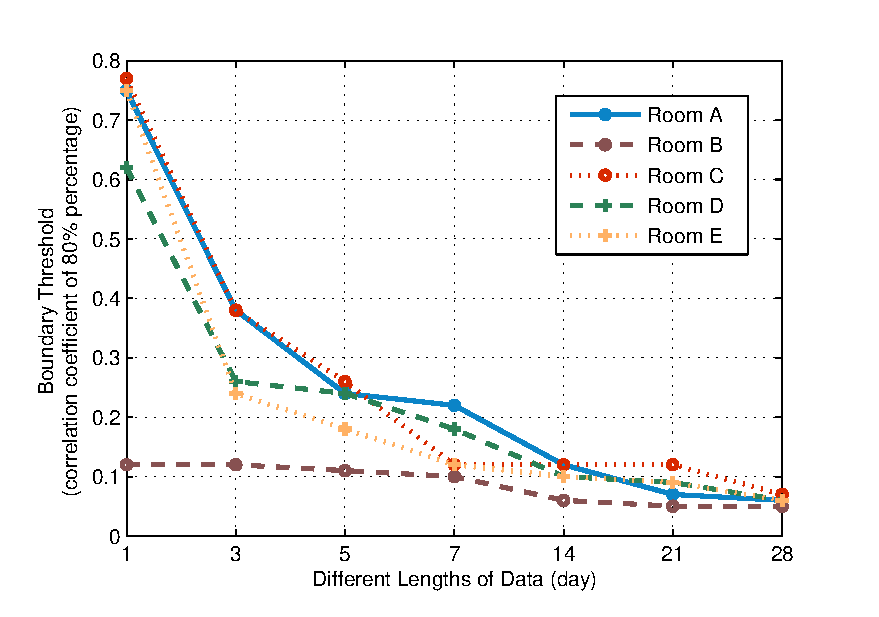
\includegraphics[width=0.48\textwidth]{./figs/lengtheffect.eps}
% \caption{The threshold values all converge to a similar value and we can derive the optimal value with as minimal as 14 days data.}
% \label{fig:leneff}
% \end{figure}

% % With the above decision on choosing the 80\% percentage corrcoeff as a threshold parameter, we also examine how the discriminator value responses to different time spans and whether the value converges as this is critical to automate the process of threshold parameter choice. 
% Using the threshold the roughly 80th-percentile corrcoeff corresponds to in the distribution, we examine how it affects the classification rate across traces
% that span different lengths of time.  Convergence and consistency across different time spans is critical to automate the parameter selection
% process.
% % To test the effect of data length on the threshold value, we use the corrcoeff distribution of sensor pairs in different rooms 
% % over different time spans and identify the 80\%-percentile corrcoeff values. 
% Observe how the  threshold values differ quite significantly in Figure~\ref{fig:leneff}.  However, 
% the threshold values 
% gradually converge, as the length of training data increases from one day to one month.  The values derived after 14 days of data
% are approximately the same as the final convergence value (around 0.07).  In other words, we can determine a threshold from two weeks of data.
% %  and cluster
% % after 14 days or longer time period, the discriminator values for all the rooms converge to almost the same point.
% \subsection{Clustering Results}
% We cluster the sensor traces over the entire one-month period, and use the roughly 80th percentile corrceff (0.07) as the boundary threshold. 
% % Note, a sensor can have corrcoeffs greater than the threshold with sensors in more than one room. When this occurs, 
% A sensor is classified into the cluster with the largest corrcoeff. The clustering result is shown in Table~\ref{tab:cluster}.  A ``1" means the sensor is classified as inside the corresponding room. 
% In general, after obtaining the sensor clusters, we don't know which room each cluster corresponds to without further information such as the metadata of sensors. The labels ``A-E" in Table~\ref{tab:cluster} are used to indicate the ground truth of where each sensor is physically placed since we have such information. Overall, the classification accuracy 
% % (defined as the number of correctly clustered sensors compared to total 
% % attempted clustering) 
% is 93.3\%.  We do not cluster on the corrcoeffs obtained among raw signals because the 80\%-percentile corrcoeff values do not converge across rooms.
% The reason that we are able to get such a high accuracy, which is seemingly different from the statistics in Figure~\ref{fig:cdf} and Figure~\ref{fig:roc}, is because the statistics in the two figures are generated out of the corrcoeffs accumulated over different time spans (the same intervals in Figure~\ref{fig:leneff}) while the clustering here is performed on the corrcoeffs from the entire one-month period. 
% % vary a lot and it doesn't make much sense to use different threshold for each room individually.

% \begin{table}[h!]\footnotesize
%  \begin{center}
% 	\begin{tabular}{ r|c|c|c|c|c|c }
% 	\multicolumn{1}{r}{}
% 	 &  \multicolumn{1}{c}{$A$}
% 	 & \multicolumn{1}{c}{$B$}
% 	 & \multicolumn{1}{c}{$C$}
% 	 & \multicolumn{1}{c}{$D$}
% 	  & \multicolumn{1}{c}{$E$} \\
% 	\cline{2-6} 
% 	$SensorA_{1}$ & 1 & 0 & 0 & 0 & 0 & \checkmark\\
% 	\cline{2-6}
% 	$A_{2}$ & 1 & 0 & 0 & 0 & 0 & \checkmark\\
% 	\cline{2-6}
% 	$A_{3}$ & 1 & 0 & 0 & 0 & 0 & \checkmark\\
% 	\cline{2-6}
% 	$B_{1}$ & 0 & 1 & 0 & 0 & 0 & \checkmark\\
% 	\cline{2-6}
% 	$B_{2}$ & 0 & 1 & 0 & 0 & 0 & \checkmark\\
% 	\cline{2-6}
% 	$B_{3}$ & 0 & 1 & 0 & 0 & 0 & \checkmark\\
% 	\cline{2-6}
% 	$C_{1}$ & 0 & 0 & 1 & 0 & 0 & \checkmark\\
% 	\cline{2-6}
% 	$C_{2}$ & 0 & 0 & 1 & 0 & 0 & \checkmark\\
% 	\cline{2-6}
% 	$C_{3}$ & 0 & 0 & 1 & 0 & 0 & \checkmark\\
% 	\cline{2-6}
% 	$D_{1}$ & 0 & 0 & 0 & 1 & 0 & \checkmark\\
% 	\cline{2-6}
% 	$D_{2}$ & 0 & 0 & 0 & 1 & 0 & \checkmark\\
% 	\cline{2-6}
% 	$D_{3}$ & 0 & 0 & 1 & 0 & 0 & $\times$\\
% 	\cline{2-6}
% 	$E_{1}$ & 0 & 0 & 0 & 0 & 1 & \checkmark\\
% 	\cline{2-6}
% 	$E_{2}$ & 0 & 0 & 0 & 0 & 1 & \checkmark\\
% 	\cline{2-6}
% 	$E_{3}$ & 0 & 0 & 0 & 0 & 1 & \checkmark\\
% 	\cline{2-6}
% 	\end{tabular}
%  \end{center}
%  \caption{Clustering result using the thresholding method: a ``1" means the sensor is classified as inside the room. We get the ``\checkmark" and ``$\times$" by comparing the clustering results with ground truth.}
%  \label{tab:cluster}
% \end{table}

% \begin{figure*}[ht!]
% \centering
% 	\begin{subfigure}{0.48\textwidth}
%                 \centering
% 		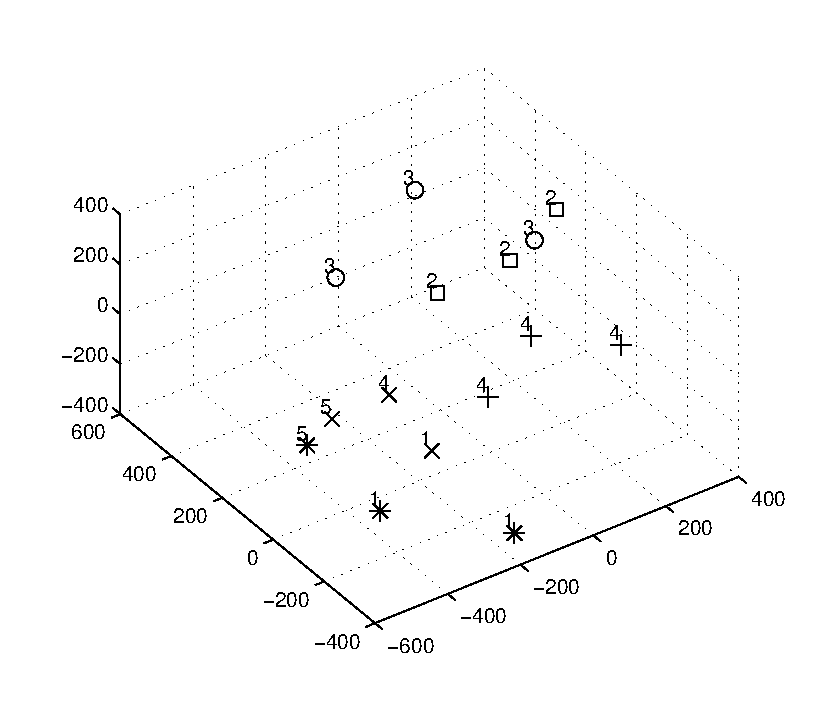
\includegraphics[width=\textwidth]{./figs/res_emd.eps}
%                 \caption{Clustering on corrcoeffs from our method.}
%                 \label{fig:res_emd}
% 	\end{subfigure}
% 	\begin{subfigure}{0.48\textwidth}
%                 \centering
% 		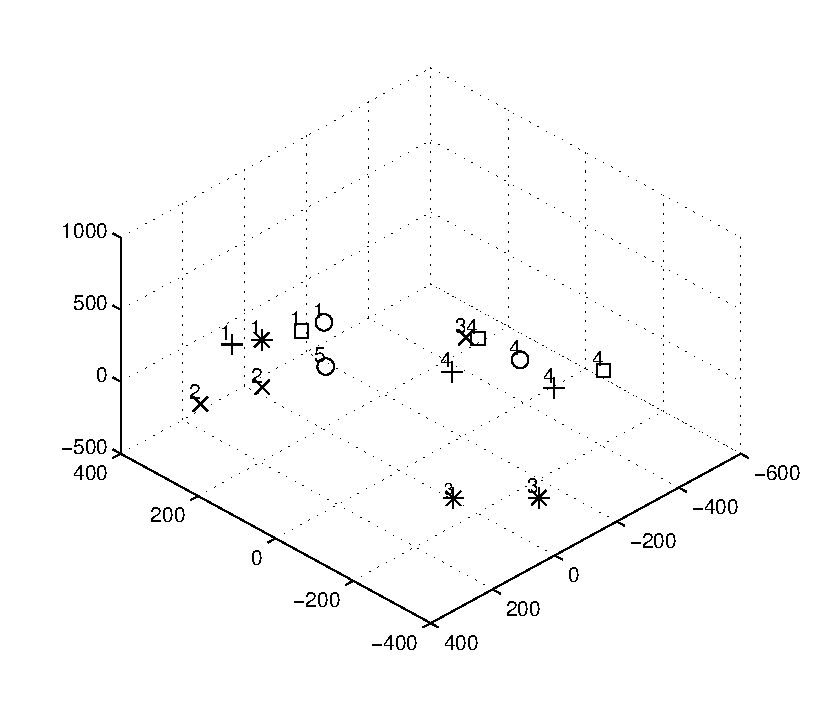
\includegraphics[width=\textwidth]{./figs/res_bsln.eps}
%                 \caption{Clustering on corrcoeffs from the naive approach.}
%                 \label{fig:res_bsln}
% 	\end{subfigure}
% \caption{Clustering with k-means on the corrcoeff matrix after applying multidimensional scaling (MDS): The EMD-based set achieves an accuracy of 80\% while the results with raw-trace is only 53.3\% classification accuracy.}
% \label{fig:mds}
% \end{figure*}

% To compare with our threshold-based method, we also cluster using a baseline approach. The pairwise corrcoeff for sensors in different rooms can be interpreted as a ``distance" between them.
% A larger coefficient indicates a closer ``distance", and vice versa.  However, since the distances between pairs is relative, we use
% multidimensional scaling~\cite{MDS} to find a common basis in three dimensions, re-map the relative distance metric (feature vector) into 
% this three-dimensional grid and use k-means to classify the traces. % assuming the value of k is known a priori, which is the number of rooms.
% We set k to equal the number of rooms, since the goal of the approach is to verify spatial placement at room-level granularity.  Generally, 
% we believe that k should equal the number of rooms you wish to classify the sensors into.
% % Such distances between points corresponds to the dissimilarities between 
% % a pair in the original high-dimensional space which is inviable to visualize. 
% %Therefore, we use Multidimensional Scaling \cite{MDS} to decrease the dimension of corrcoeff matrix to a 3-D space and use k-means to do the clustering. 
% The clustering results are shown in Figure~\ref{fig:mds}.  Ground truth is shown through different markers (x, o, +, star, box). Each marker stands for one room. 
% The cluster each sensor assigned to is denoted with a number. The classification accuracy of the baseline approach on corrcoeffs matrix of re-aggregated IMFs is 80\%. 
% For raw traces, the baseline approach achieves an accuracy of only 53.3\%.





\subsection{Categorical Properties}

\begin{enumerate}
\item Soda Hall data (ART, OAT, VAV, RVAV)
\item Todai data
\item KETI data
\end{enumerate}

\subsection{Methodology}

\subsection{Results}


%\begin{figure*}[htb!]
%\begin{center}
%\includegraphics[width=18cm]{../figs/channel_comp}
%\caption{RSSI measurements for specific channels over time. The values are averaged over a minute. Most sensor networks are set to channel 26 to minimize chance of interference, but in this case, channel 15 is significantly better}
%\label{channelcomp}
%\end{center}
%\end{figure*}



\newpage

\section{Discussion}
\subsection{Applications}
\subsection{Future Work}

\newpage


\section{Conclusion}
\label{sec:conc}




\vspace{+0.5mm}
\vspace{+2mm}
%\bibliographystyle{IEEETran}
\bibliographystyle{sig-alternate}
%\bibliographystyle{abbrv}
%\scriptsize
\bibliography{references}
%\bibliography{references}

\end{document}


